\documentclass[11pt,a4paper]{article}
\usepackage[margin=2.2cm]{geometry}
\usepackage[T1]{fontenc}
\usepackage{lmodern}
\usepackage{microtype}
\usepackage{amsmath}
\usepackage{booktabs}
\usepackage{tabularx}
\usepackage{xcolor}
\usepackage{tikz}
\usetikzlibrary{arrows.meta,positioning}
\usepackage{listings}
\usepackage[hyphens]{url}
\usepackage{hyperref}
\usepackage{enumitem}
\setlist{nosep,leftmargin=1.4em}

\definecolor{shared}{HTML}{DBEAFE}
\definecolor{sharededge}{HTML}{1D4ED8}
\definecolor{head}{HTML}{FEF3C7}
\definecolor{headedge}{HTML}{B45309}
\definecolor{io}{HTML}{F1F5F9}
\definecolor{ioedge}{HTML}{475569}
\definecolor{codebg}{HTML}{F8FAFC}
\hypersetup{colorlinks=true,linkcolor=sharededge,urlcolor=sharededge}

\lstset{basicstyle=\ttfamily\small,backgroundcolor=\color{codebg},frame=single,
  rulecolor=\color{ioedge!40},breaklines=true,columns=fullflexible,keepspaces=true}

\tikzset{
  box/.style={draw=ioedge,fill=io,rounded corners=3pt,align=center,font=\small,inner sep=4pt,minimum height=9mm},
  sbox/.style={draw=sharededge,fill=shared,rounded corners=3pt,align=center,font=\small,inner sep=4pt,minimum height=9mm},
  hbox/.style={draw=headedge,fill=head,rounded corners=3pt,align=center,font=\small,inner sep=4pt,minimum height=9mm},
  arr/.style={-{Stealth[length=2mm]},thick,draw=ioedge},
}

\newcolumntype{L}{>{\raggedright\arraybackslash}X}

\title{\textbf{Decide, explained from zero}\\[2pt]\large What it does, how it works, and how it was tested}
\author{Amal Verma}
\date{October 2026}

\begin{document}
\maketitle
\noindent A plain-language guide to the project. Read this first if you are new to it.
The technical write-up is in \texttt{report.pdf}.

\section{The problem}
Support software makes many small decisions on every ticket: which team should handle
it, whether a refund can be auto-approved, and whether the drafted reply is backed by
the help article. Many products ask a large LLM these questions. That is slow (0.3 to
2\,s), costs money per call, and comes back with no usable confidence. The hackathon
asks for a \textbf{small model} that answers these typed questions in one pass, on a
CPU, in milliseconds, with an honest probability.

\section{Input and output}
You send one ticket and name \textbf{one} question:
\begin{lstlisting}
{ "request_id": "demo-1",
  "decision": "approve",
  "state": {
    "subject": "Refund for last month",
    "body": "Hi, I was charged $45.00 for a month I didn't use. Can you refund it?",
    "customer_tier": "pro",
    "amount": 45.0,
    "draft_reply": "You can request a refund within 60 days of the charge on any plan. Once approved, the money goes back to your original payment method within 10 business days.",
    "kb_article": "Refunds may be requested within 30 days of the charge, and this applies to all plans. Approved refunds are returned to the original payment method within 10 business days." } }
\end{lstlisting}

\noindent\begin{tabularx}{\linewidth}{@{}lL@{}}
\toprule
Field & Meaning \\
\midrule
\texttt{subject}, \texttt{body} & what the customer wrote \\
\texttt{customer\_tier} & free, pro or enterprise \\
\texttt{amount} & money involved \\
\texttt{draft\_reply} & a reply someone drafted \\
\texttt{kb\_article} & the help article that reply should rely on (\textbf{given in the request}; we never search for it) \\
\bottomrule
\end{tabularx}

\medskip
\noindent The same ticket, asked all three questions (real output of the served model):

\medskip
\noindent\begin{tabularx}{\linewidth}{@{}lp{4.6cm}L@{}}
\toprule
Question & Output & Meaning \\
\midrule
\texttt{route} & \texttt{billing}, confidence 0.888, abstain true, plus probabilities for all 5 queues & billing, 89\% sure; just under the 0.892 bar, so a human confirms \\
\texttt{approve} & \texttt{true}, $p$ = 0.883, abstain false & auto-approve: pro tier, \$45 is under the about \$120 limit, no red flags \\
\texttt{grounded} & \texttt{false}, $p$ = 0.055, abstain true & the draft says 60 days; the article says 30 \\
\bottomrule
\end{tabularx}

\medskip
\noindent Every answer has \texttt{value} (the answer), \texttt{probs} or \texttt{p\_true}
(the honest probability), \texttt{abstain} (true means ``let a human check'') and
\texttt{latency\_ms}.

\section{The rules that make it hard}
\begin{enumerate}
  \item \textbf{One model for all three questions}, sharing a backbone; not three models behind a switch.
  \item \textbf{CPU only, no network} while answering.
  \item \textbf{Fast}: p95 under 100\,ms; full marks at 25\,ms or less.
  \item \textbf{Calibrated}: ``0.8'' must be right about 80\% of the time.
  \item \textbf{Can abstain}, but must answer at least 80\%.
  \item \textbf{Approve has a 3:1 cost}: a wrong approval costs 3 times a wrong hold.
  \item \textbf{The approve rule is secret}: it must be learned from the labels, and part of it depends on account history the ticket never shows.
\end{enumerate}

\paragraph{Point 6: why approve uses 0.75, not 0.5.} At probability $p$ that the request
is fine, approving costs $3(1-p)$ on average and holding costs $p$. They are equal at
$3(1-p) = p$, so $p = 0.75$. The model approves only above 0.75. For example, at $p = 0.6$
approving costs 1.2 and holding costs 0.6.

\paragraph{Point 7: the rule recovered from the data.}
\begin{center}
\begin{tabular}{lc}
\toprule
Tier & usually auto-approved up to \\
\midrule
free & about \$30 \\
pro & about \$120 \\
enterprise & about \$500 \\
\bottomrule
\end{tabular}
\end{center}
Red flags force a hold at any amount: ``raised something similar'', ``signed up
recently'', ``disputed a charge with my bank'', ``outside your usual policy\ldots{} an
exception''. Even when everything looks fine, about 20\% of such tickets are still held
because of hidden account history. The model says about 0.85 on those, which is honest.

\section{How it is scored}
Pass/fail first: valid schema on every response, p95 under 100\,ms, a model card, and no
memorising dev. Then teams are ranked on a hidden test set:

\medskip
\noindent\begin{tabularx}{\linewidth}{@{}llL@{}}
\toprule
Axis & Weight & Meaning \\
\midrule
Quality & 40\% & right answers on the cases you answered (route and grounded macro-F1, approve 3:1 cost) \\
Calibration & 25\% & half ECE (is 0.8 really 0.8?), half Brier skill (better than quoting the base rate?) \\
Latency & 20\% & p95 per call; full marks at 25\,ms or less \\
Abstention & 15\% & does your confidence point at your own mistakes? \\
\bottomrule
\end{tabularx}

\section{The architecture, step by step}
The served model is an \textbf{ensemble}: two complete models that each answer all three
questions, packed into \textbf{one} ONNX file and computed in \textbf{one} call.

\begin{center}
\resizebox{\linewidth}{!}{%
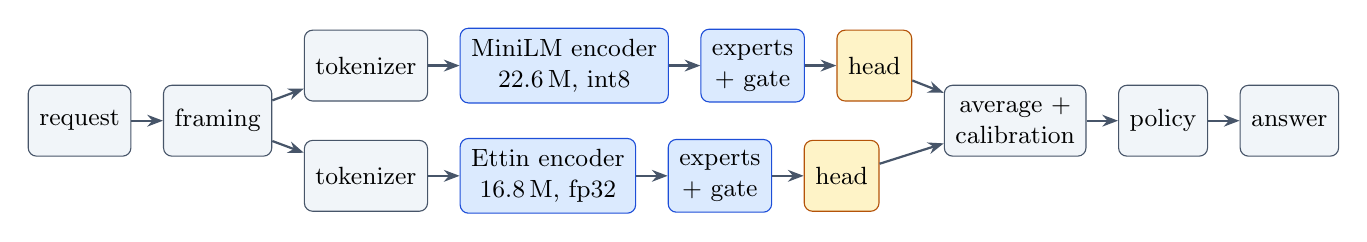
\begin{tikzpicture}[node distance=4mm]
  \node[box] (a) {request};
  \node[box, right=of a] (b) {framing};
  \node[box, right=of b, yshift=7mm] (c1) {tokenizer};
  \node[box, right=of b, yshift=-7mm] (c2) {tokenizer};
  \node[sbox, right=of c1] (d1) {MiniLM encoder\\22.6\,M, int8};
  \node[sbox, right=of c2] (d2) {Ettin encoder\\16.8\,M, fp32};
  \node[sbox, right=of d1] (e1) {experts\\+ gate};
  \node[sbox, right=of d2] (e2) {experts\\+ gate};
  \node[hbox, right=of e1] (f1) {head};
  \node[hbox, right=of e2] (f2) {head};
  \node[box, right=of f1, yshift=-7mm] (g) {average +\\calibration};
  \node[box, right=of g] (h) {policy};
  \node[box, right=of h] (i) {answer};
  \foreach \x/\y in {a/b,b/c1,b/c2,c1/d1,c2/d2,d1/e1,d2/e2,e1/f1,e2/f2,f1/g,f2/g,g/h,h/i} \draw[arr] (\x) -- (\y);
\end{tikzpicture}}
\end{center}
\noindent Blue parts are shared by all three questions inside each member; the amber
heads are per question.

\begin{enumerate}
  \item \textbf{Framing} (\texttt{decide/inputs.py}). Each question sees what it needs.
        Route reads subject + body. Approve reads ``pro plan, amount \$45. subject'' + body,
        plus numbers for tier, amount above each cutoff and red flags. Grounded reads
        kb\_article + draft\_reply side by side, plus numbers for whether the durations match.
  \item \textbf{Tokenizers.} Words become IDs. Each member has its own dictionary
        (\texttt{artifacts/tok\_m}, \texttt{artifacts/tok\_e}).
  \item \textbf{Encoders.} Every word looks at every other word (attention), so meaning
        comes from context. The output is averaged into one summary. Member 1 is MiniLM
        (6 layers, 384 numbers wide, 22.6\,M weights, stored as int8). Member 2 is
        Ettin-17m (7 layers, 256 wide, 16.8\,M weights, kept at full precision).
        \textbf{Each encoder is shared by all questions.}
  \item \textbf{Mixture of experts}, one per member (4 expert layers + a gate). The gate
        decides how much to trust each expert for this question. \textbf{Shared.}
  \item \textbf{Heads.} One tiny layer per question per member gives the raw score: route
        5 scores (1{,}285 weights), approve 1 score (257), grounded 1 score (257). This is
        the only per-question part.
  \item \textbf{Averaging and calibration.} Each member's raw score is divided by its own
        temperature, the two are averaged, and the average is divided by a final
        temperature (route 1.00, approve 0.96, grounded 0.84). Softmax (route) or sigmoid
        (binary) then gives honest probabilities.
  \item \textbf{Policy} (\texttt{model.py}): commit to an answer and decide whether to
        abstain (Section~\ref{sec:abstain}).
\end{enumerate}
\noindent\textbf{Size:} about 40.2\,M parameters (23.07\,M MiniLM member + 17.17\,M Ettin
member), over 99.99\% shared across the three questions. That is about 10 times smaller
than the 421\,M Laya model the brief mentions.

\paragraph{Why two members?} They make different mistakes, so averaging helps. In 4-fold
cross-validation the pair scored 83.13\,$\pm$\,0.53 against 82.57\,$\pm$\,1.29 for MiniLM
alone. The price is about twice the latency.

\section{How \texttt{grounded} is calculated}
Same article as in Section 2, three drafts, real numbers from the served model:

\medskip
\noindent\begin{tabularx}{\linewidth}{@{}Lrrrp{3.2cm}@{}}
\toprule
Draft & MiniLM raw & Ettin raw & $p$ & Why \\
\midrule
faithful rewrite: 30 days, any plan, 10 business days & $+11.91$ & $+13.10$ & 1.00 & everything is supported \\
same, but ``60 days'' & $-1.90$ & $-3.70$ & 0.06 & wrong number \\
same, but ``3 business days'' & $-6.96$ & $-13.58$ & 0.00003 & wrong number \\
\bottomrule
\end{tabularx}

\medskip
\noindent For the ``60 days'' draft: MiniLM $-1.90 \div 1.216 = -1.56$ and Ettin
$-3.70 \div 1.149 = -3.22$; their average is $-2.39$; divided by the final temperature
0.842 that is $-2.84$, and the sigmoid of $-2.84$ is 0.055. The value is $0.055 > 0.5$,
which is false. Abstain asks whether $\max(0.055, 0.945) < 0.9957$, which is true.

\paragraph{What it misses.} Drafts that invent an action (``so I have put yours
through'') or narrow the scope (``but only on the enterprise plan'') were both scored as
grounded ($p$ about 1.00). The model learned the kinds of mismatch in the training data,
which are mostly changed numbers.

\section{Abstention}\label{sec:abstain}
Abstention is the model saying ``not sure, let a human decide''. It works in two separate
ways:
\begin{itemize}
  \item \textbf{The \texttt{abstain} flag} sets what you are graded on. Abstained cases
        leave the quality score, but answering under 80\% scales quality down. Ours answers
        about 85\%.
  \item \textbf{The abstention score} ignores the flag. Judges sort every case by your
        confidence, keep the top 80\%, and compare the error there with the error overall.
\end{itemize}

\begin{center}
\begin{tabular}{lcc}
\toprule
Decision & error, all cases & error, most confident 80\% \\
\midrule
route & 10.7\% & 5.1\% \\
approve & 10.5\% & 6.0\% \\
grounded & 1.2\% & 0.08\% \\
\bottomrule
\end{tabular}
\end{center}
Our abstention score is 0.63. It is capped by noisy labels and hidden account history:
some mistakes look certain because nothing in the ticket reveals them.

Thresholds (\texttt{artifacts/policy.json}): route abstains when its top probability is
under 0.892; grounded when it is under 99.57\% sure either way; approve when
$0.15 < p < 0.79$. That band is lopsided because risky approvals are the costly mistakes.

\section{Training}
\begin{enumerate}
  \item 6{,}500 tickets from \texttt{train.jsonl}: 5{,}500 to train, 1{,}000 held out (the
        same rows for both members). \textbf{Dev is never used for training or fitting.}
  \item Each ticket becomes 3 training items (one per question), 16{,}500 in total.
  \item Batches of 32 items from one question pass through the model. The error (loss)
        is measured and all the member's weights are nudged to reduce it. Because the
        encoder is shared, every question improves the same brain.
  \item 5 passes over the data, seed 13, on a free Kaggle T4 GPU. This is done twice,
        once per member. The Ettin member is a deterministic rerun of an earlier run;
        three reruns reproduced it exactly.
  \item Temperatures and abstain thresholds are fitted on the 1{,}000 held-out
        tickets (\texttt{fit\_ensemble.py}).
  \item Export to ONNX. MiniLM is compressed to int8; Ettin stays fp32. The two are merged
        into one graph.
\end{enumerate}

\section{fp32 against int8}
\begin{center}
\begin{tabular}{lcc}
\toprule
 & fp32 (32-bit) & int8 (8-bit, quantized) \\
\midrule
bytes per weight & 4 & 1 \\
used for & training, and the served Ettin member & the served MiniLM member \\
\bottomrule
\end{tabular}
\end{center}
int8 makes a model about 4 times smaller and usually faster, at a small cost in accuracy.
For MiniLM the cost is tiny: int8 and fp32 give the same answer on 99.7 to 100\% of cases.
For Ettin it is not: they agree on only 91\% of route, 92\% of approve and 81\% of
grounded cases. An ensemble with Ettin in int8 scored 82.24 on dev; with Ettin at fp32 it
scored 85.44. So Ettin ships at fp32, and the merged file is 92\,MB.

\begin{itemize}
  \item \textbf{The served ensemble} (MiniLM int8 + Ettin fp32): the official dev score
        85.44, latency, the schema check and the demo.
  \item \textbf{fp32} (predictions saved during GPU training): cross-validation, the
        second split, and the backbone and policy experiments.
\end{itemize}

\section{Was it tested on other splits?}
\begin{center}
\noindent\begin{tabularx}{\linewidth}{@{}lL@{}}
\toprule
Test & Result \\
\midrule
dev split (served ensemble, never trained on dev) & \textbf{85.44} \\
dev split, MiniLM member alone & 83.75 \\
4-fold CV of the ensemble (fresh fp32 models per fold) & 83.13 $\pm$ 0.53 \\
4-fold CV, MiniLM alone (same folds) & 82.57 $\pm$ 1.29 \\
4-fold CV, shuffle B (stopped early; accuracy only) & route 0.885 to 0.895, approve 0.894 to 0.909, grounded 0.973 to 0.977 \\
\bottomrule
\end{tabularx}
\end{center}
The ensemble's dev gain (+1.69) is larger than its cross-validated gain (+0.56), so
part of the dev 85.44 is a favourable Ettin run. The honest expected hidden-test score is
roughly 83 to 85. Most of the spread comes from approve, the noisiest label.

\section{Key decisions}
\noindent\begin{tabularx}{\linewidth}{@{}lL@{}}
\toprule
Decision & Why \\
\midrule
ensemble of MiniLM and Ettin-17m & best and steadiest in cross-validation (83.13 $\pm$ 0.53); costs about 2 times the latency, still under 25\,ms p95 \\
Ettin kept at fp32 & int8 changed up to 19\% of its answers \\
small H384 encoder over the larger H768 & H768 grounds slightly better but is about 1.7 times slower, which risks the latency score \\
never train on dev & keeps dev scores honest and respects the ``no memorising dev'' rule \\
lopsided approve abstention band & a wrong approval costs 3 times a wrong hold \\
5 epochs, 85\% coverage target & best and safest settings in cross-validation \\
\bottomrule
\end{tabularx}

\end{document}
